\chapter{Optimal Portfolio Allocation}
\label{chpr:markowitz}

In this chapter we will explore what the optimal allocation is for our portfolio of assets. We will study the \textit{efficient frontier} using two different risk measures, volatility and expected shortfall. In all our analyses, we will be comparing the effects that including Bitcoin in our portfolio has on the optimal allocation.


\section{Markowitz Mean-Variance Portfolio Optimization}
\label{sec:markowitz_theory}

Modern Portfolio Theory (MPT) is a mathematical framework for creating a portfolio of asset by maximizing the expected return for a given level of risk or by minizing the risk while maintaining the same expected gain. 
Before the article \citep{MARKOWITZ1952} by Harry Markowitz in 1952, the concept of \textit{diversification} (the old warning \textit{not to put all your eggs in one basket}) was only driven by the experience of how markets behave.
Moreover, investors used to base their decisions on expected return alone and thus when given a choice between two assets with different expected returns, they would put all their money on the top performing one.

With his article, that would later grant him the Nobel Prize in Economics, Markowitz introduced a more rigorous and mathematically sound framework to assembly a portfolio of assets. His key insight is that an asset's return and risk risk should not be assessed by itself, but rather by how it affects the overall portfolio risk and return.
To do so, the \textit{variance} is used as a proxy for risk. Hence the name \textit{mean-variance } analysis that is often used as a substitute for MPT.

\bigskip
Let's introduce the assumption underlying the MPT:
\begin{enumerate}
	\item Investors are \textit{risk averse}: they will always choose the less risky asset, when two assets offer the same return.  At the same time, an investor wanting a higher return has to be willing to accept a higher risk.
	This equally holds for portfolios as a whole: given two portfolio with the different risk profiles, he will choose the less risky in case of same return and the most remunerating in case of same risk.
	\item Portfolio return is the weighted sum of the single assets' returns: in general $\mathbb{E}[R_{ptf}] = \sum_{i=1}^{N} w_i \mathbb{E}[R_i]$.
	\item Portfolio variance is a function of both the assets variances and their correlations: $V_{ptf} = \sum_{i=1}^{N} w_i \sigma_i^2 + \sum_{i=1}^{N}\sum_{j\neq i , j=1}^{N} w_i w_j \rho_{i,j}\sigma_i\sigma_j$
\end{enumerate}

Items 2 and 3 above can be more compactly stated using matrix notation, which will come in handy later on in our analysis:
\begin{equation}
\label{eq:ptf_return}
r_{ptf}(\mathbf{w}) = \mathbf{w}^T \mathbf{r}
\end{equation}
\begin{equation}
\label{eq:sigma_ptf}
	\sigma^2_{ptf}(\mathbf{w}) =  \mathbf{w}^T \Sigma \mathbf{w}
\end{equation}

where we have the weights vector $\mathbf{w} = [w_1, w_2, ... , w_N]^T$ , $\mathbf{r} = [r_1, r_2, ... , r_N]^T$, using the shorthand $r_i = \mathbb{E}[R_i]$ and finally $\Sigma$ is the $N\times N$ covariance matrix of the assets.

\bigskip

We can now state the \textit{optimization problem} involving the minimization of the portfolio risk for a specified expected portfolio return in terms of the variable we have just introduced.

\begin{subequations}
	\label{eq:markowitz_opt}
	\begin{align}
%	\label{eq:mark_min}
	&\!\min_{\mathbf{w}\in \mathbb{R}^{N}}     &    & \sigma^2_{ptf}(\mathbf{w}) \\
%	\label{eq:mark_weights}
	& \text{subject to}   &   & \mathbf{e}^T\mathbf{w} = 1 ,\\
%	\label{eq:mark_return}
	&                 &       & \mathbf{r}^T\mathbf{w} = r_{target},\label{eq:constraint2a} \\
%	\label{eq:mark_noshort}
	&		   &      & w_{i} \geq 0, \text{for} \: i = 1\dots N. 
	\end{align}
\end{subequations}

where \textbf{e} indicates a vector of ones and the first constraint makes sure that the sum of the weights always equals to one. This is to represent a portfolio in which all the money available is allocated in the assets we are taking into consideration.
The second constraint ensures that the portfolio allocation $\mathbf{w}$ produces the target expected return $r_{target}$.
Finally, the last constraint is in fact optional and is only used to exclude the possibility to go short on any asset.

The optimization problem in \eqref{eq:markowitz_opt} has a quadratic objective function given by \eqref{eq:sigma_ptf} and only has linear constraints\footnote{The last positivity constraint can be easily expressed in matrix form by writing $ \mathbf{I}_N\mathbf{w} \geq \mathbf{0}_N$ where $\mathbf{I}_N$ is the identity matrix of order $N$ and $\mathbf{0}_N$ is N-dimensional vector of zeros.}. Thanks to this property, the optimization can be carried out numerically by any of the quadratic/linear optimizers that are available for most programming languages.

As we are going to explain in the following sections, we will be mainly focusing on the case where there is no short selling, as indeed so far there are no instruments on the market that allow an investor to go short on Bitcoin and our analysis shows that the main diversification advantage comes from including Bitcoin in our portfolio. Allowing short-selling improves our diversification capability only so slightly.



\section{Markowitz Efficient Frontier}
\label{sec:markowitz_frontier}

It is interesting to study the set of optimal allocation as a whole, rather than simply focus on one target return and minimizing the portfolio risk.
To do so, we can consider a set of target returns and compute for each of them the respective minimum variance. We thus get a set of pairs $(\sigma^2, r)$ that represents the best allocation in terms of the minimum risk.

We can thus plot those pairs on an X-Y graph and obtain a curve, the \textit{portfolio frontier}, that intrinsically represents our portfolio of $N$ assets.
As a usual practice in finance, we will be plotting on the X-axis the volatility $\sigma$ instead of the variance $\sigma^2$.

\begin{figure}
	\centering
	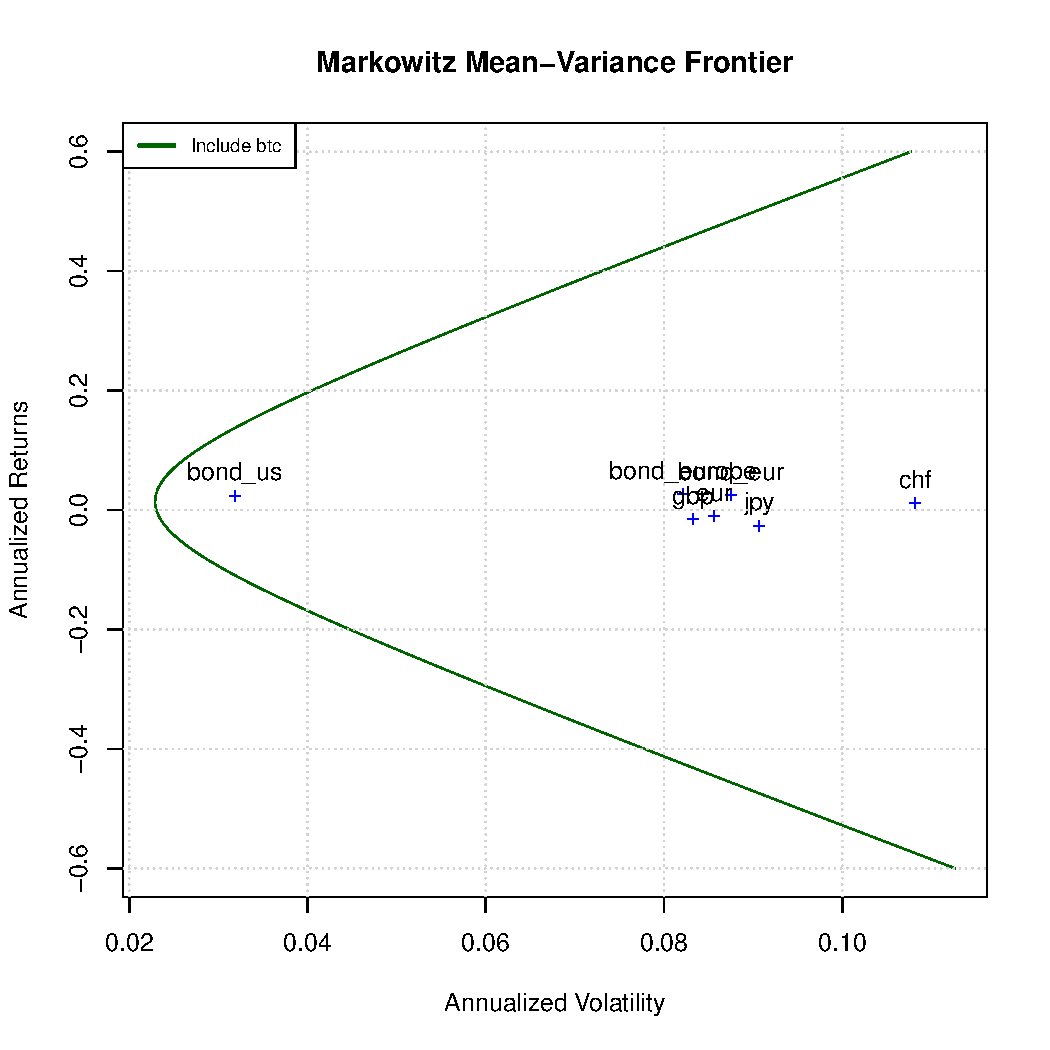
\includegraphics[width=0.6\textwidth]{Images/full_frontier.pdf}
	\caption[Full Markowitz Efficient Frontier]{The Markowitz Mean-Variance frontier obtained from our portfolio of assets, that includes Bitcoin and allows short-selling.}
	\label{fig:full_frontier}
\end{figure}

In Figure \ref{fig:full_frontier} we can see what the portfolio frontier looks like for our portfolio of assets. 
It is interesting to notice how the curve divides the plane in two region: the area to the left of the line includes all those pairs $(\sigma, r)$ that are not attainable with our assets, since they have a volatility that is too low for that level of expected return. On the other hand, the region to the right of the portfolio frontier is made of all the pairs that are possible to obtain with a specific allocation $\mathbf{w}$ but that will never be chosen by an investor: moving to the left on the same level of return we eventually reach a point on the frontier. The portfolio represented by this point will dominate the one we started from in terms of risk, so it will always be a better choice.

We can proceed with the same argument arguing in terms of best return for a given level of risk: we can thus introduce the \textit{efficient} frontier. For every level of volatility that has two corresponding points on the portfolio frontier, only the one with the higher expected return will be chosen by an investor in our reference framework: hence only the top half of the curve (from the vertex and up) will form the \textit{efficient portfolio frontier}.

As a summary, let us keep in mind that any point in the volatility-expected return plane \textit{dominates} all the other portfolio allocations that are represented by points situated below and to the right of it. Conversely, that same point will be dominated by all other allocations above and to the left of it. 

Another mathematical perk of considering only the efficient top section is that it renders the frontier a \textit{bijective} function. Hence, for each (attainable) level of risk there is one and only one corresponding expected portfolio return, and vice-versa.


\subsection{Efficient Frontier with and without Bitcoin}

Let us now study how including Bitcoin in our portfolio of assets can help increase the diversification and obtain a higher (expected) return with a lower risk.

In Figure \ref{fig:efficient_frontier_comparison} we have plotted the efficient Markowitz frontier in all possible cases: including and excluding Bitcoin while allowing short-selling, and the same two curves when short-selling is not allowed.

Comparing the two green lines, we can clearly see that the exclusion of short-selling does not penalize our efficient allocation by much. The same can be stated for the red and orange curves, which represent our portfolio when excluding the digital asset.
Thus, given our particular set of assets, allowing for short-selling does very little to improve the diversification of our portfolio.

Let us now take a look of what happens when we include Bitcoin in the reference portfolio: as we can see from Figure \ref{fig:efficient_frontier_comparison}, we get a significant improvement in the expected return when considering each level of risk . Equivalently, for the same level of return we have a noticeable decrease in the volatility of our portfolio.

\textbf{***AGGIUNGERE COMMENTO INCISIVO***}
%This is indeed one of the main result of this work

We can see some numerical proof of the diversification properties of adding Bitcoin to our portfolio in Table \ref{tab:markowitz_ret_on_vol} and Table	\ref{tab:markowitz_vol_on_ret}.

\begin{table}
	\centering
	\caption[Markowitz efficient frontier on volatility]{Expected return for different levels of volatility, both including and excluding Bitcoin.}
	\label{tab:markowitz_ret_on_vol}
\begin{tabular}{ccc}

Volatility Level & Return without Bitcoin & Return including Bitcoin \\
\midrule
2.61\% & 3.00\% & 3.00\% \\
2.75\% & 3.89\% & 7.70\% \\
3.00\% & 4.59\% & 10.94\% \\
3.25\% & 5.05\% & 13.37\% \\
3.50\% & 5.43\% & 15.48\% \\
3.75\% & 5.76\% & 17.41\% \\
4.00\% & 6.06\% & 19.21\% \\
4.25\% & 6.34\% & 20.94\% \\
4.50\% & 6.61\% & 22.60\% \\
4.75\% & 6.87\% & 24.21\% \\
5.00\% & 7.12\% & 25.79\% \\
5.25\% & 7.37\% & 27.34\% \\
5.50\% & 7.61\% & 28.86\% \\
5.75\% & 7.85\% & 30.37\% \\
6.00\% & 8.08\% & 31.85\% \\
\midrule
\end{tabular}
\end{table}

\begin{table}
	\centering
	\caption[Markowitz efficient frontier on returns]{Volatility for different level of expected portfolio return, both including and excluding Bitcoin.}
	\label{tab:markowitz_vol_on_ret}
\begin{tabular}{ccc}
	Return Level & Volatility without Bitcoin & Volatility including Bitcoin\\
	\midrule
	3.00\% & 2.61\% & 2.61\% \\
	3.50\% & 2.61\% & 2.67\% \\
	4.00\% & 2.61\% & 2.78\% \\
	4.50\% & 2.62\% & 2.96\% \\
	5.00\% & 2.63\% & 3.22\% \\
	5.50\% & 2.65\% & 3.55\% \\
	6.00\% & 2.67\% & 3.95\% \\
	6.50\% & 2.69\% & 4.40\% \\
	7.00\% & 2.71\% & 4.88\% \\
	7.50\% & 2.74\% & 5.39\% \\
	8.00\% & 2.77\% & 5.91\% \\
	8.50\% & 2.80\% & 6.45\% \\
	9.00\% & 2.84\% & 7.00\% \\
	9.50\% & 2.88\% & 7.56\% \\
	10.00\% & 2.92\% & 8.12\% \\
	10.50\% & 2.96\% & 8.69\% \\
	11.00\% & 3.01\% & 9.27\% \\
	11.50\% & 3.05\% & 9.85\% \\
	12.00\% & 3.10\% & 10.43\% \\
	12.50\% & 3.16\% & 11.01\% \\
	13.00\% & 3.21\% & 11.60\% \\
	13.50\% & 3.26\% & 12.19\% \\
	14.00\% & 3.32\% & 12.78\% \\
	14.50\% & 3.38\% & 13.37\% \\
	15.00\% & 3.44\% & 13.96\% \\
	\midrule
\end{tabular}

\end{table}


\begin{figure}
	\centering
	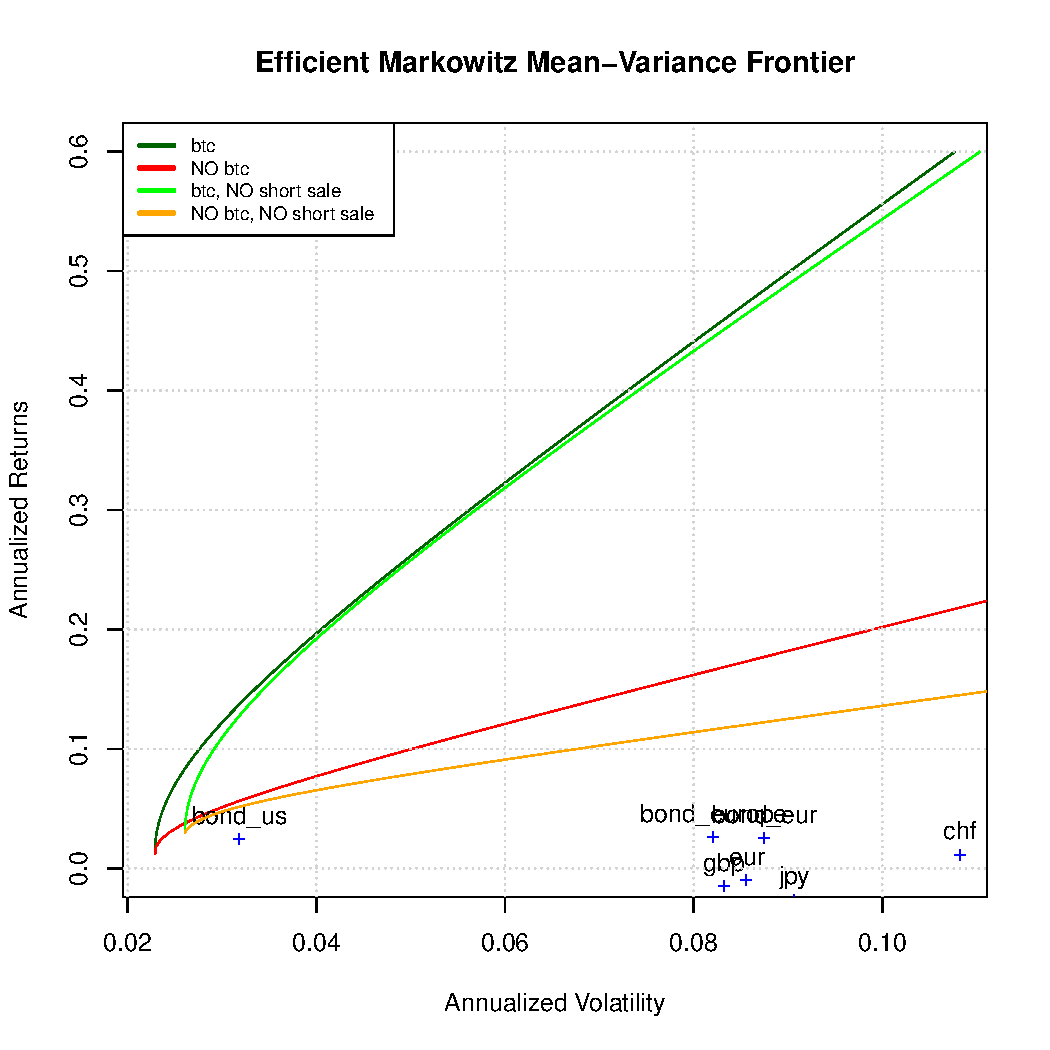
\includegraphics[width=0.6\textwidth]{Images/efficient_frontier.pdf}
	\caption[Markowitz Efficient frontier comparison]{The \textit{Efficient} Markowitz Mean-Variance frontier obtained from our portfolio of assets, both including and excluding Bitcoin and with short-selling or not.}
	\label{fig:efficient_frontier_comparison}
\end{figure}


\subsection{Portfolio Allocation}
We have so far seen the implications of introducing the digital asset in our portfolio in terms of improvement in the expected return and of lowering the overall portfolio risk.
Let us now take a look at how Markowitz MPT allocates the wealth into the different assets.

To do so, we can plot the values of $\mathbf{w}$ as resulting from \eqref{eq:markowitz_opt} for different levels of returns (and hence volatilities): resulting allocations are plotted in Figure \ref{fig:markowitz_allocation}.


\begin{figure}
	\centering
\begin{subfigure}{0.8\textwidth}
	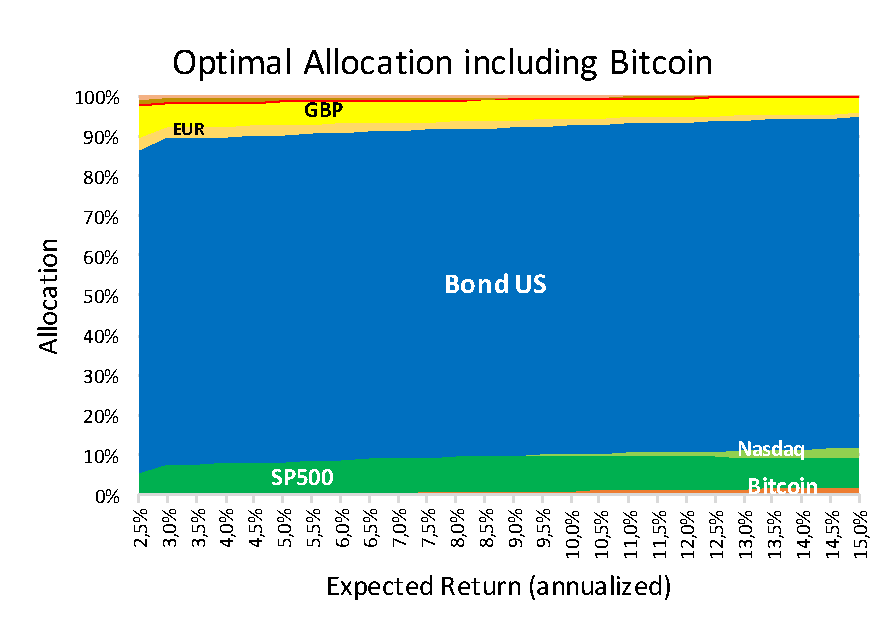
\includegraphics[width=\linewidth]{Images/markowitz_allocation}
	\caption{Allocation including Bitcoin.}
\end{subfigure}

\begin{subfigure}{0.8\textwidth}
	\centering
	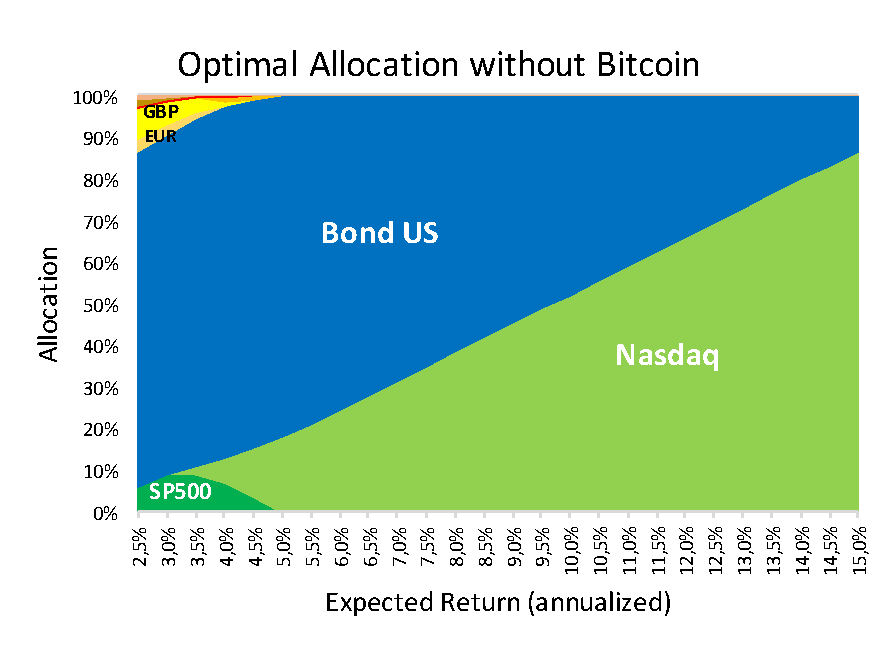
\includegraphics[width=\linewidth]{Images/markowitz_allocation_no_btc}
	\caption{Allocation without Bitcoin.}
\end{subfigure}
\caption[Markowitz Optimal Allocations]{The figures represent the composition of the portfolio for different levels of expected returns, both including and excluding Bitcoin.  The percentage of wealth invested in Bitcoin is about 1.5\%  for  10\% expected return and  2\% for 15\%. Respective values of portfolio volatility can be found in Table \ref{tab:markowitz_vol_on_ret}.}
\label{fig:markowitz_allocation}
\end{figure}





\section{Portfolio Optimization with CVaR as a Risk Measure}
\label{sec:cvar_theory}

We have so far studied the problem of optimal portfolio allocation through Markowitz MPT, considering the portfolio volatility as a proxy for its risk.
This is only one of the possible choices in a more general framework in which the optimization problem to be solved maintains the same constraints but has a  different objective function. We can reformulate \eqref{eq:markowitz_opt} as follows:

\begin{subequations}
	\label{eq:general_opt}
	\begin{align}
	%	\label{eq:mark_min}
	&\!\min_{\mathbf{w}\in \mathbb{R}^{N}}     &    & PtfRisk(\mathbf{w}) \\
	%	\label{eq:mark_weights}
	& \text{subject to}   &   & \mathbf{e}^T\mathbf{w} = 1 ,\\
	%	\label{eq:mark_return}
	&                 &       & \mathbf{r}^T\mathbf{w} = r_{target},\label{eq:constraint2} \\
	%	\label{eq:mark_noshort}
	&		   &      & w_{i} \geq 0, \text{for} \: i = 1\dots N. 
	\end{align}
\end{subequations}

where we have substituted the portfolio volatility with a general measure of the portfolio risk as a function of the weights $\mathbf{w}$.

Using the portfolio volatility as risk measure has its perks and downsides: it is an intuitive and simple way to evaluate how the possible returns vary from the expected value but it takes into account both the positive and the negative deviation from the mean. Thus, a high volatility may be caused by a few extremely high returns that are anything but something to avoid and penalize.
For this reason, the notion of \textit{semi-volatility} was introduced to only consider variations towards lower returns than the one expected. This solution however is not very popular.

A more common approach is to measure risk based on the quantile of the loss distribution \footnote{Depending on how the returns are expressed, we have different ways to compute the loss. In particular, considering the time interval $[0, T]$, for log-returns $r_{log}=log(S_T/S_0)$ the loss is simply the opposite $Loss_{log} = - r_{log}$ while for $r_\% = S_T/S_0$  the loss is $Loss_\% = 1 - r_\%$. As usual we indicate by $S_t$ the price  of the asset or the value of the portfolio at time $t$.}. The \textit{Value-at-Risk} of level $\alpha$ for a loss distribution is precisely defined as the quantile of order $\alpha$ \footnote{ There are two different notations when it comes to what the number $\alpha$ indicates. In this work, $\alpha$ is considered as the percentage of losses that are lower or equal to the value of $VaR_\alpha$. The other notation is to consider $\alpha$ as the percentage of losses that exceed the $VaR_\alpha$. }.  In formulas, $VaR_\alpha$ is the value such that:
\begin{equation}
\mathbb{P}(Loss \leq VaR_\alpha) = \alpha
\end{equation}
VaR is a vastly popular and common way to measure the so called ``tail-risk'': the intrinsic risk contained in loss events that happen very rarely. 
Its advantage is that it considers only the downside of the expected return as opposed to what the volatility does.

However, VaR has drawbacks as its mathematical definition does not make it a \textit{coherent measure of risk}. Specifically, it lacks the property of sub-additivity: the VaR of two different portfolios  considered as one may be greater than the sum of the two single VaRs. This is in direct contradiction with the principle of diversification.

\textbf{aggiungere appendice dove si definisce una misura coerente di rischio con le 3/4 proprieties}

An improved version of VaR is the \textit{Conditional Value-at-Risk} (CVaR), also referred to as \textit{expected shortfall} since indeed it is defined as the average loss among the values of the loss distribution that exceed the corresponding VaR level. Thus, for a continuous loss distribution is defined as:
\begin{equation}
	CVaR_\alpha = \frac{1}{1-\alpha} \int_{\alpha}^{1} VaR_\gamma d\gamma 
\end{equation}

There are two advantages in the usage of CVaR as opposed to VaR. Firstly, it can be proven that CVaR is a \textit{coherent} measure of risk, so we gain an important mathematical property that before was lacking. Secondly, we now take into account also the very extreme values that a loss distribution might have. The latter is especially true for discrete loss distributions (e.g. losses obtained from daily assets returns, which will is our main focus) since there might be a very few  truly high losses that nonetheless will be considered in the computation of CVaR. On the other hand, the VaR for discrete distributions just amounts to sorting all the possible losses in increasing order and taking the element in position $100*\alpha / N_{sample}$ as our $VaR_\alpha$. 

These are the reasons that induced us to consider the CVaR as an alternative measure of portfolio risk to be inserted as the objective function to be minimized in the optimization problem \eqref{eq:general_opt}. 
Considering the literature, there are already a few studies in which the conditional value at risk is used in the optimal portfolio allocation problem,  above all the paper by Rockafellar and Uryasev in \citep{ROCKAFELLAR2000}. Following studies include for instance in \citep{DICLEMENTE2002} and \citep{QUARANTA2008}. 
Most of these approaches are based on continuous loss functions, and as a further study beyond this work it could be of interest to study the diversification effect of the inclusion of Bitcoin in the assets portfolio in those frameworks. As we are about to see, our approach  focuses on optimizing the empirical historical CVaR from daily return data.




\section{CVaR Efficient Frontier}
\label{sec:cvar_frontier}

Following a similar approach to the one we developed in previous sections regarding Markowitz optimization, we will now present the CVaR efficient frontier.

\subsection{Efficient Frontier with and without Bitcoin}


In order to perform an  analysis similar to what we have done using Markowitz approach in the case of the daily CVaR as the portfolio risk measure, we have to solve the following optimization problem:

\begin{subequations}
	\label{eq:general_opt_CVaR}
	\begin{align}
	%	\label{eq:mark_min}
	&\!\min_{\mathbf{w}\in \mathbb{R}^{N}}     &    & PtfCVaR_\alpha^{daily}(\mathbf{w}) \\
	%	\label{eq:mark_weights}
	& \text{subject to}   &   & \mathbf{e}^T\mathbf{w} = 1 ,\\
	%	\label{eq:mark_return}
	&                 &       & \mathbf{r}^T\mathbf{w} = r_{target},\label{eq:constraint2b} \\
	%	\label{eq:mark_noshort}
	&		   &      & w_{i} \geq 0, \text{for} \: i = 1\dots N. 
	\end{align}
\end{subequations}

To compute the daily CVaR of the portfolio, we considered the daily percentage returns for all the assets and all the time-steps available, and stored them in matrix $R$. $R$ has dimension $N_{timesteps} \times N_{assets}$. We then obtained the distribution of returns for a portfolio with weights $\mathbf{w}$ by doing $R_{ptf}(\mathbf{w}) = R \mathbf{w} $. The CVaR is now computed as explained in the previous section.

We computed the efficient frontier for the two usual portfolios: one that includes Bitcoin and the other that only contains \textit{standard} assets, both without short-selling. The graphs for both frontiers are plotted in Figure \ref{fig:cvar_efficient_frontier_comparison}.


\begin{figure}
	\centering
	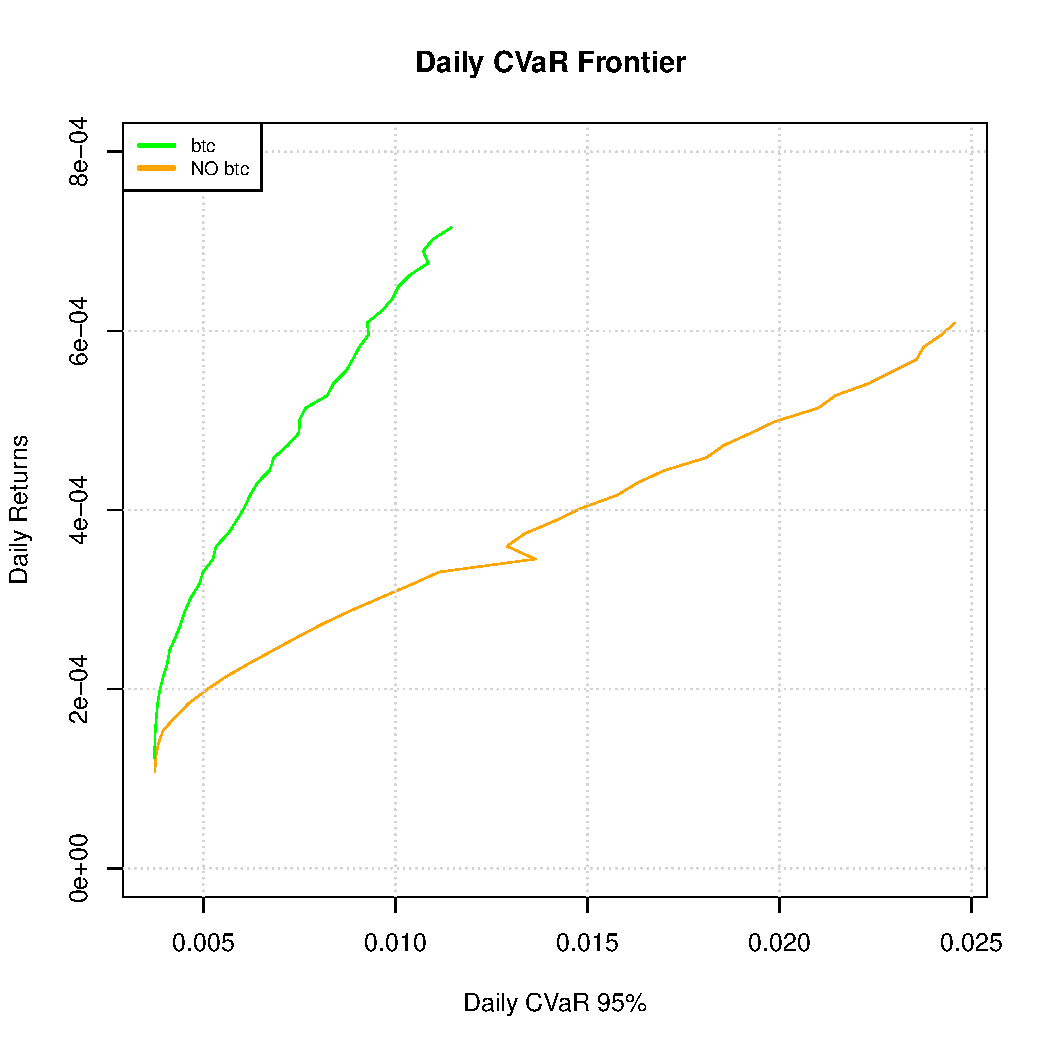
\includegraphics[width=0.6\textwidth]{Images/efficient_frontier_CVaR.pdf}
	\caption[Efficient CVaR frontier comparison]{The \textit{Efficient} daily $CVaR_{95\%}$ frontier obtained from our portfolio of assets, both including and excluding Bitcoin and without short-selling.}
	\label{fig:cvar_efficient_frontier_comparison}
\end{figure}


At first glance, we notice that both curves are not perfectly smooth: this is due to the fact that we are using the \textit{discrete} historical distribution for the returns of the assets. On the contrary, when we set our analysis in the MPT framework it can be shown that the optimal frontier has the shape of a hyperbole when allowing short-selling. Without short sales, the frontier is no longer a hyperbole but it is still a smooth function.

The improvement in portfolio diversification when including Bitcoin in our basket is clearly visible in how the two efficient frontiers part from each other, in the same way that they did in Figure \ref{fig:efficient_frontier_comparison}.
We can easily tell from the picture that for the same level of return an investor has to be willing to risk losing more money (higher CVaR) when he does not include Bitcoin in his portfolio of asset.
Similarly, for a given level of risk, including the digital asset in our basket allows for a significant increase in the daily expected return,  hence also for a higher annual profit.

Numerical results for this section are given in Table \ref{tab:return_cvar}.

\begin{table}
	\centering
	\caption[CVaR efficient frontier on returns]{Results for the optimal daily portfolio CVaR of level $95\%$ for a number of daily expected returns, both including and excluding Bitcoin from our basket.}
	\label{tab:return_cvar}
\begin{tabular}{ccc}
	
	Daily Return & $DailyCVaR_{95\%}$ without Bitcoin & $DailyCVaR_{95\%}$ including Bitcoin \\
	\midrule
	0.012\% & 0.376\% & 0.373\% \\
	0.014\% & 0.383\% & 0.374\% \\
	0.015\% & 0.396\% & 0.375\% \\
	0.017\% & 0.425\% & 0.377\% \\
	0.018\% & 0.457\% & 0.381\% \\
	0.020\% & 0.505\% & 0.387\% \\
	0.021\% & 0.560\% & 0.394\% \\
	0.023\% & 0.617\% & 0.406\% \\
	0.024\% & 0.684\% & 0.411\% \\
	0.026\% & 0.753\% & 0.423\% \\
	0.027\% & 0.870\% & 0.436\% \\
	0.029\% & 0.883\% & 0.455\% \\
	0.030\% & 0.973\% & 0.472\% \\
	0.032\% & 1.026\% & 0.487\% \\
	0.033\% & 1.121\% & 0.495\% \\
	0.035\% & 1.190\% & 0.528\% \\
	0.036\% & 1.256\% & 0.536\% \\
	0.037\% & 1.334\% & 0.565\% \\
	0.039\% & 1.403\% & 0.585\% \\
	0.040\% & 1.478\% & 0.595\% \\
	0.042\% & 1.557\% & 0.612\% \\
	0.043\% & 1.637\% & 0.643\% \\
	0.044\% & 1.700\% & 0.679\% \\
	0.046\% & 1.787\% & 0.689\% \\
	0.047\% & 1.870\% & 0.699\% \\
	0.049\% & 1.936\% & 0.729\% \\
	0.050\% & 2.036\% & 0.763\% \\
	0.051\% & 2.077\% & 0.767\% \\
	0.053\% & 2.152\% & 0.802\% \\
	0.054\% & 2.241\% & 0.820\% \\
	0.056\% & 2.295\% & 0.831\% \\
	0.057\% & 2.361\% & 0.882\% \\
	0.058\% & 2.386\% & 0.892\% \\
	0.060\% & 2.421\% & 0.918\% \\
	0.061\% & 2.448\% & 0.950\% \\
	\midrule
\end{tabular}

\end{table}

\subsection{Portfolio Allocation}
We have seen again the implications of introducing the digital asset in our portfolio in terms of improvement in the expected return and of lowering the daily CVaR of the portfolio.
Let us now take a look at how this second type of optimization allocates the money in the different assets.

To do so, we will plot the values of $\mathbf{w}$ as resulting from \eqref{eq:general_opt_CVaR} for different levels of daily CVaR (and hence returns).


\begin{figure}
	\centering
	\begin{subfigure}{0.8\textwidth}
		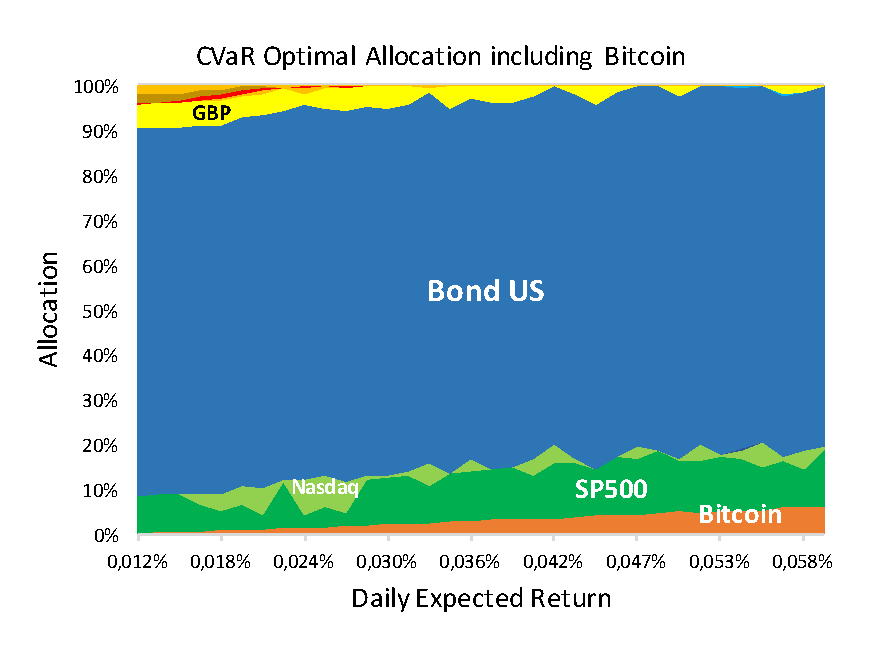
\includegraphics[width=\linewidth]{Images/cvar_allocation}
		\caption{Allocation including Bitcoin.}
	\end{subfigure}
	
	\begin{subfigure}{0.8\textwidth}
		\centering
		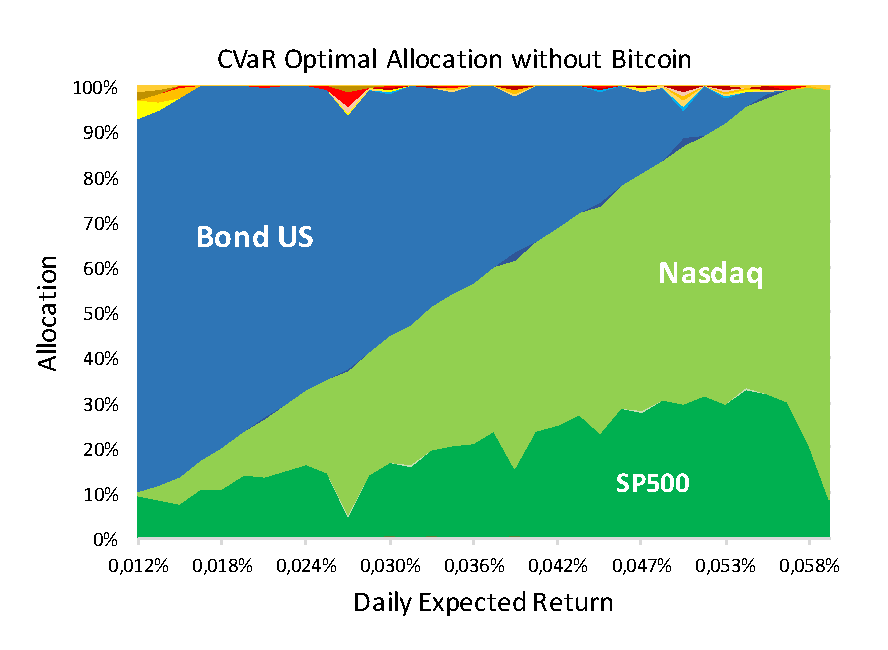
\includegraphics[width=\linewidth]{Images/cvar_allocation_no_btc}
		\caption{Allocation without Bitcoin.}
	\end{subfigure}
	\caption[CVaR Optimal Allocations]{The figures represent the composition of the portfolio for different levels of expected returns, both including and excluding Bitcoin.  The percentage of wealth invested in Bitcoin is about 3\%  for  0.036\% expected daily return and  about 6\% for 0.058\%. Respective values of portfolio volatility can be found in Table \ref{tab:return_cvar}.}
	\label{fig:markowitz_allocation}
\end{figure}
